\documentclass[10pt]{article}
\usepackage[polish]{babel}
\usepackage[utf8]{inputenc}
\usepackage[T1]{fontenc}
\usepackage{amsmath}
\usepackage{amsfonts}
\usepackage{amssymb}
\usepackage[version=4]{mhchem}
\usepackage{stmaryrd}
\usepackage{graphicx}
\usepackage[export]{adjustbox}
\graphicspath{ {./images/} }

\title{GIMNAZJUM }

\author{}
\date{}


\begin{document}
\maketitle
\begin{enumerate}
  \item Udowodnij, że pole trójkąta można policzyć ze wzoru:
\end{enumerate}

\[
P=r_{a}(p-a)
\]

gdzie \(r_{a}\) oznacza promień okręgu dopisanego do trójkąta, stycznego do boku długości \(a\), a \(p\) oznacza połowę obwodu.\\
2. Czworokąt \(A B C D\) ma kąty proste przy wierzchołkach \(B\) i \(D\). Ponadto \(A B=B C\) i \(B H=1\). Oblicz pole tego czworokąta.\\
3. W puste pola wpisz takie cyfry, aby spełnione były wszystkie równości. Żadna z liczb w rebusie nie może zaczynać się zerem.\\
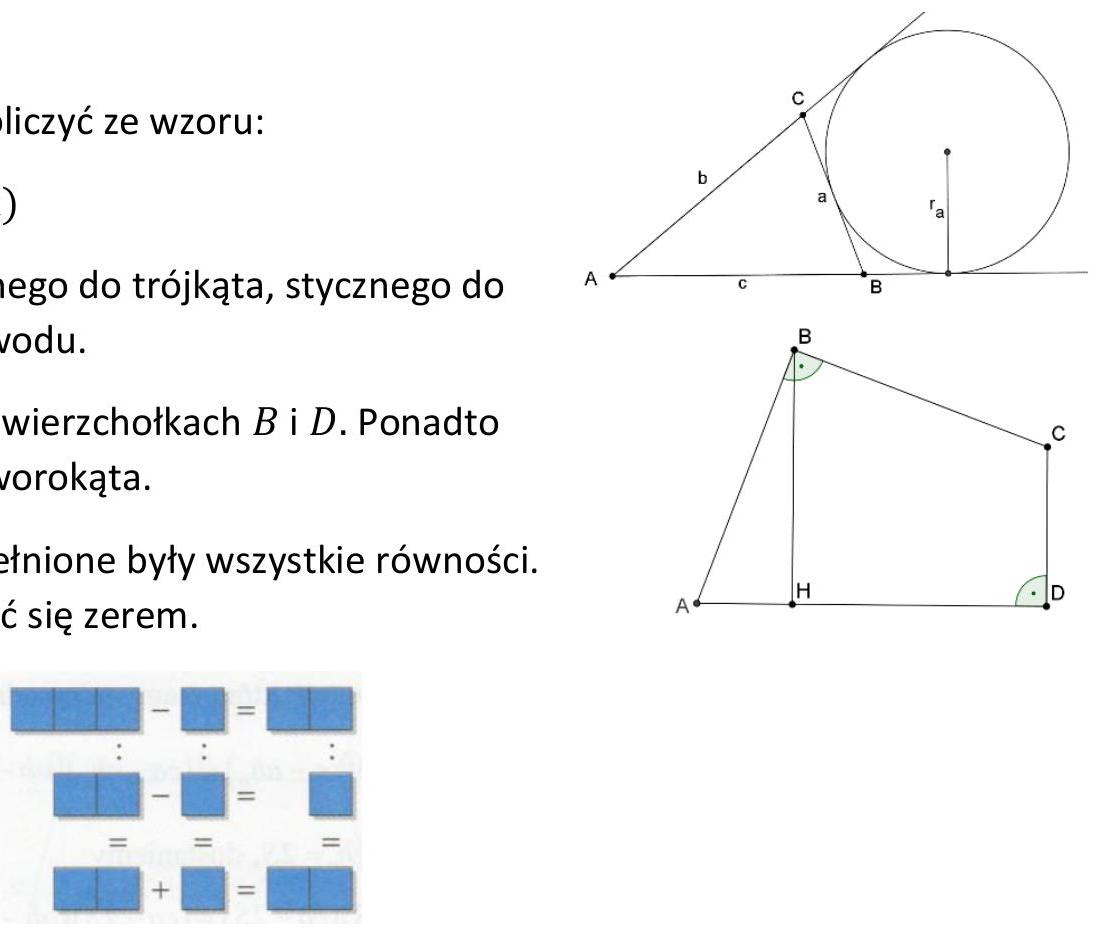
\includegraphics[max width=\textwidth, center]{2024_11_21_f4c7fc65cc2b3b951b8fg-1}

\section*{LICEUM}
\begin{enumerate}
  \item Udowodnij tożsamość \(\frac{1}{r_{a}}+\frac{1}{r_{b}}+\frac{1}{r_{c}}=\frac{1}{r}\), gdzie \(r_{a}, r_{b}, r_{c}\) oznaczają promienie okręgów dopisanych do trójkąta \(A B C\), a \(r\) oznacza promień okręgu wpisanego w ten trójkąt. Możesz skorzystać z zadania 1 dla gimnazjum.
  \item Przekątna czworokąta wypukłego połowi odcinek łączący środki dwóch przeciwległych boków tego czworokąta. Udowodnij, że przekątna ta połowi także pole tego czworokąta.
  \item Liczby od 1 do 9 wpisz w kółeczka figury\\
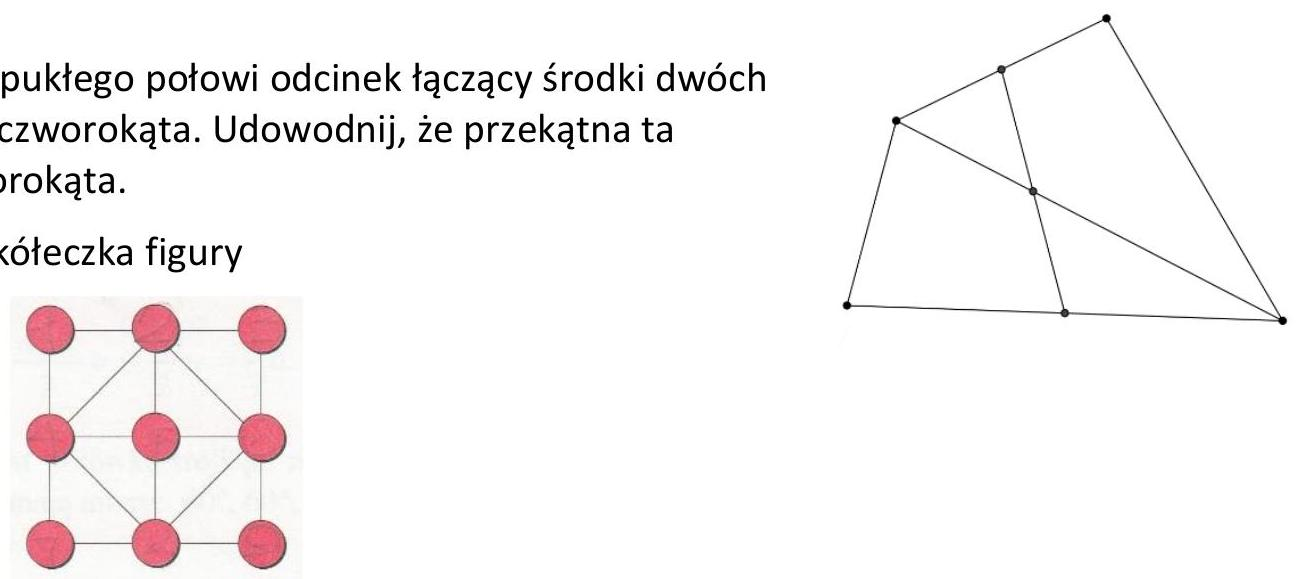
\includegraphics[max width=\textwidth, center]{2024_11_21_f4c7fc65cc2b3b951b8fg-1(1)}\\
tak, aby sumy czterech liczb w kółeczkach - wierzchołkach wszystkich kwadratów, były równe.
\end{enumerate}

\end{document}